This section details the web interface layer and the three subsystems that it encompasses. The web interface layer includes the login, feedback and arrow key interface subsystems.


In this section, the layer is described in some detail in terms of its specific subsystems. Describe each of the layers and its subsystems in a separate chapter/major subsection of this document. The content of each subsystem description should be similar. Include in this section any special considerations and/or trade-offs considered for the approach you have chosen.

\subsection{Login Subsystem}
The login sybststen will receive internet access from the black box system and be the first interface that the user will arrive at. The user will be required to access the system using a password or username stored in a database on the Raspberry Pi.

\begin{figure}[h!]
	\centering
 	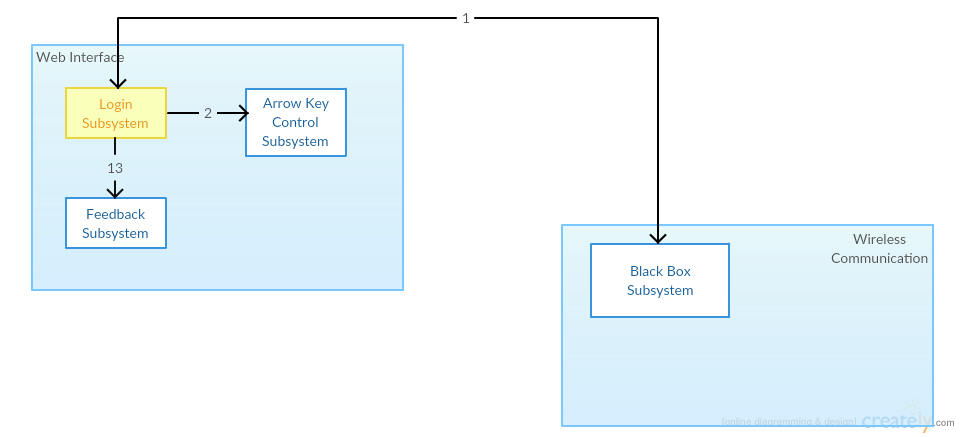
\includegraphics[width=0.60\textwidth]{images/ADSdiagrams/login_subsystem.png}
 \caption{Diagram of the Login Subsystem}
\end{figure}

\subsubsection{Assumptions}
The login subsystem relies on an internet connection to allow users to connect to it and access the camera feed.

\subsubsection{Responsibilities}
Each of the responsibilities/features/functions/services of the subsystem as identified in the architectural summary must be expanded to more detailed responsibilities. These responsibilities form the basis for the identification of the finer-grained responsibilities of the layer's internal subsystems. Clearly describe what each subsystem does.

\subsubsection{Login Subsystem  Interfaces}

\begin {table}[H]
\caption {Login Subsystem Interfaces} 
\begin{center}
    \begin{tabular}{ | p{1cm} | p{6cm} | p{3cm} | p{3cm} |}
    \hline
    ID & Description & Inputs & Outputs \\ \hline
    \#1 & The interface between the blackbox and the login system provides an internet connection so the user can communicate with the web interface.  & \pbox{3cm}{Incoming internet connection and the user's username and password} & \pbox{3cm}{Validation or rejection of the username and a redirection to the cameras feed if successful}  \\ \hline
    \#2 & This interface is reached after a successful validaion from the login system. & \pbox{3cm}{N/A} & \pbox{3cm}{The login system redirects the user to the Arrow Key Control Subsystem}  \\ \hline
    \#13 & The login system redirects to the feedback system on successful validaion. & \pbox{3cm}{N/A} & \pbox{3cm}{Validation of user login and redirect to }  \\ \hline	
    \end{tabular}
\end{center}
\end{table}


\subsection{Arrow Key Control Subsystem}
The arrow key control subsystem is reached after a successful validation from the login subsystem and provides the ability to pan and tilt the camera.

\begin{figure}[h!]
	\centering
 	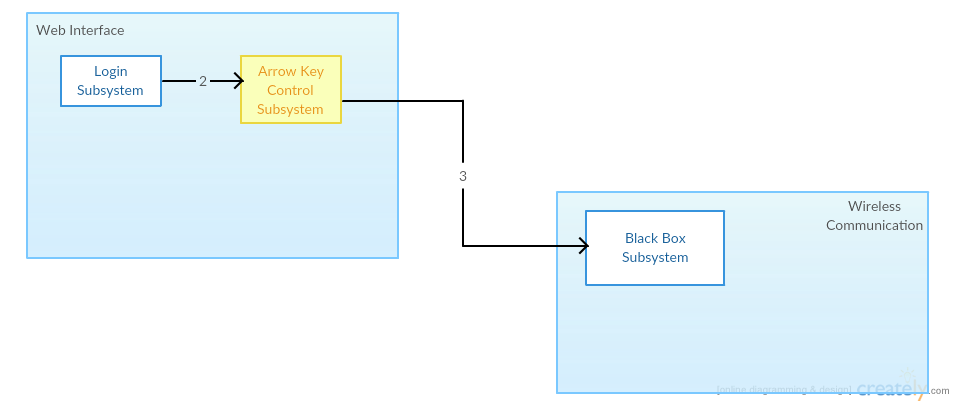
\includegraphics[width=0.60\textwidth]{images/ADSdiagrams/arrow_key_control_subsystem.png}
 \caption{Diagram of the arrow key control subsystem}
\end{figure}

\subsubsection{Assumptions}
The arrow key control subsystem assumes the user has been validated by the login subsystem.

\subsubsection{Responsibilities}
The arrow key control subsystem is responsible for ensuring that the user is able to control the camera's pan and tilt functionality, which includes relaying commands to the respective stepper motors.

\subsubsection{Arrow Key Control Subsystem Interfaces}

\begin {table}[H]
\caption {Arrow Key Control Interfaces} 
\begin{center}
    \begin{tabular}{ | p{1cm} | p{6cm} | p{3cm} | p{3cm} |}
    \hline
    ID & Description & Inputs & Outputs \\ \hline
    \#2 & This interface is reached after a successful validaion from the login system. & \pbox{3cm}{Successful validation and a redirect to the arrow key control subsystem} & \pbox{3cm}{N/A}  \\ \hline
    \#3 & The interface between the blackbox and the arrow key control subsystem provides an internet connection so the user can communicate with the web interface.  & \pbox{3cm}{N/A} & \pbox{3cm}{Control of the camera's stepper motors and verification to the user that the camera responded via the blackbox subsystem.}  \\ \hline

    \end{tabular}
\end{center}
\end{table}


\subsection{Feedback Subsystem Subsystem}
The feedback subsystem is responsible for relaying the camera feed back to the user once they have been successfully validated by the login subsystem.

\begin{figure}[h!]
	\centering
 	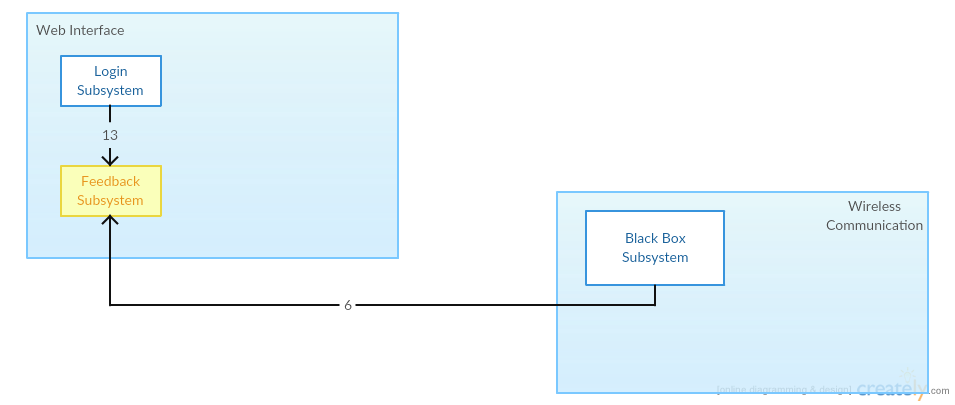
\includegraphics[width=0.60\textwidth]{images/ADSdiagrams/feedback_subsystem.png}
 \caption{Diagram of the feedback subsystem}
\end{figure}

\subsubsection{Assumptions}
The feedback subsystem assumes the user has been validated by the login subsystem and that the camera is operational.

\subsubsection{Responsibilities}
The feedback subsystem is responsible for fetching the current image from the camera and relaying that information back to the user.

\subsubsection{Feedback Subsystem Interfaces}

\begin {table}[H]
\caption {Feedback Interfaces} 
\begin{center}
    \begin{tabular}{ | p{1cm} | p{6cm} | p{3cm} | p{3cm} |}
    \hline
    ID & Description & Inputs & Outputs \\ \hline
 \#13 & The interface between the blackbox and the feedback subsystem provides an internet connection so the feedback subsystem can send back the requested image to the user.  & \pbox{3cm}{N/A} & \pbox{3cm}{The request image feed of the camera.}  \\ \hline
    \#13 & This interface is reached after a successful validaion from the login system. & \pbox{3cm}{Successful validation and a redirect to the feedback subsystem} & \pbox{3cm}{N/A}  \\ \hline
   
    \end{tabular}
\end{center}
\end{table}
